\section{\systemname - A Tool for Pipe Design}

Pipe design is non-trivial.  Independent pipes cannot intersect lest their contents be unintentionally mixed.  Pipes' bending energy needs to be minimized to allow easy insertion of media post-print.  Pipes in general need to avoid objects' surfaces to prevent fluid leakage when printed by hobbyist-grade machines.  Finally, for designing pipes that follow a user-specified path, we must ensure certain characteristics of that path (e.g., that the path is connected). \george{pipes are hard.  not sure we convinced readers by now that they are worth the effort.  maybe this has to happen more in the intro.  the example objects section is still a few pages away.}

To allow makers to design novel objects with pipe-powered interfaces, we created a tool for use on arbitrary 3D models.  This tool allows designers to select exterior connection points of their pipes (see Figure \ref{fig:tool-process-interior}) or to import vector art describing the pipes' interior paths (see Figure \ref{fig:tool-process-exterior}).  Once the maker's selections are made, we create a complete routing using either the exterior connection point method (A*, physical simulation) or the interior path method (graph edge creation, Euler tour generation).  We thicken our routing to create pipes.  The resultant pipes are subtracted from the original mesh, which can then be 3D printed.

Our tool is implemented as a part of Meshmixer, a consumer 3D mesh editing tool, in C++ \cite{Schmidt-meshmixer}.

\subsection{Exterior Terminals}

Designing objects which, for example, are touch sensitive in particular areas or integrate with existing electronics, requires precise location and sizing of pipe endpoints.  The interior of these pipes should have as large a bending radius as possible so that post-print insertion of solid or viscous media is easier.

To create pipes in which the location and shape of exterior connection points matters, we first allow makers to select the connection points on the mesh's surface.

\begin{figure}[h!]
\centering
    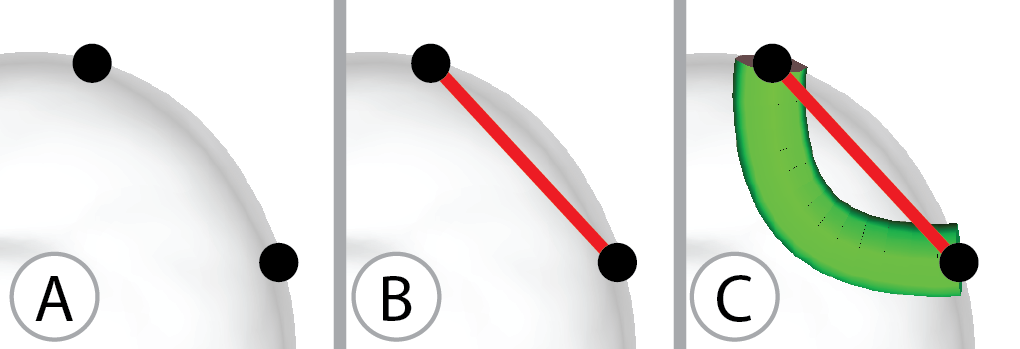
\includegraphics[width=3.4in]{figures/exterior.png}
\caption{An example mesh with exterior connection points selected.  The smoothed A* routing is drawn in {\color{red}red}, and in {\color{tovi}green} is our physically-based rod after simulation.}
\label{fig:tool-process-exterior}
\end{figure}

\subsubsection{Routing and Physical Simulation}

Our basic first-pass routing algorithm uses the A* routing algorithm \cite{Hart-Astar}.  This algorithm keeps a priority queue of points to check for routing based on a cost function; for each point it tags the distance from the start (e.g., startPoint = 0, startNeighbors=1, ...).  Once the end point is reached, we backtrack through tagged points, always moving to a lower-valued point.  The path cost in our implementation is based only on shortest distance between the starting and ending points, without weighting for distance from the surface, however the routed path is forced to stay inside the mesh's boundaries.  We route on the voxelized 3D grid of the mesh, using a resolution of 128x128x128 voxels. 

Pipes avoid each other in this manner: pipes once cut are ``outside the mesh'' and therefore not part of valid routes.  However, we do not currently track all pipes for global optimization: we greedily select the best routing per pipe.

Our A* pathfinding produces the \emph{shortest} path, but in many cases
we require a smoother path through which we can actually push a physical wire.
We solve this problem via physical simulation. We create a straight virtual 
wire (a 3D poly-line or \emph{discrete rod}), and then set its initial position 
as our A* path.
Running the physical simulation allows the wire to attempt to return to
a straight configuration, while satisfying the user-selected endpoint position constraints.
We also increase the length of the wire, to provide some slack in cases where 
it would otherwise bend sharply to stay inside the shape. 

The wire is modelled as a \emph{discrete rod}, i.e., a 3D poly-line with a bending 
constraint between adjacent segments. Our simulation is based on an
implementation of Position-Based Dynamics \cite{Muller07}, with all constraints
modelled as penalty forces. To keep the rod inside the
mesh, we compute a discretized distance field, we can then constrain the
rod to stay within some offset shell, again using a simple penalty force.
In the case of multiple initial paths, we solve for each smoothed path sequentially.
After solving for a path, we add it as a constraint to the system, generating
a penalty force that pushes additional paths away from it.

This basic approach does have various limitations, in particular it
cannot recover if the discrete rod becomes tangled or unstable. 
However we have observed these problems only when attempting to break
the system; they did not occur in any of the cases shown in our figures.
Another issue is parameters, as the penalty forces used in PBD do not
correspond to physical units. We avoided serious issues here by uniformly
scaling the initial mesh to a unit box, and tuning the parameters on several test cases.
PBD simulations rarely converge to a steady state, 
so we simply halt after a fixed number of timesteps (250). 
The simulation is very fast so this only takes a second for most of our examples.


\subsubsection{Pipes with Multiple Endpoints}
To allow designers to create pipes with multiple endpoints (e.g., star topologies in Figure \ref{fig:toys}), we use one surface position per pipe and a central fixed endpoint that the user can interactively position.  The user can connect several  then route the pipes as normal.

\subsection{Interior Paths}

In pipes where interior path layout matters, such as the neon sign in Figure \ref{fig:tool-process-interior} or the maze in Figure \ref{fig:maze}, we must create a single long path which passes through all desired path segments (i.e., all letters in the word ``UIST'' or all paths in the maze).  We built a tool which leverages graph theory to generate this single long path.

In graph theory, a semi-Eulerian graph is one which has exactly two edges of odd degree.  This kind of graph supports an Euler tour: a path that travels every edge exactly once, beginning and ending at the two nodes of odd degree (in this case, the user-selected start and end nodes).  A maker can import a vector graphics file (such as SVG) describing the path she desires for her pipes.  We create a graph based on this input data, then add edges to make it connected and semi-Eulerian.  We create an Euler tour on the modified graph, and thicken the path to create pipes.  We then cut these pipes from the mesh.

\begin{figure}[h!]
\centering
    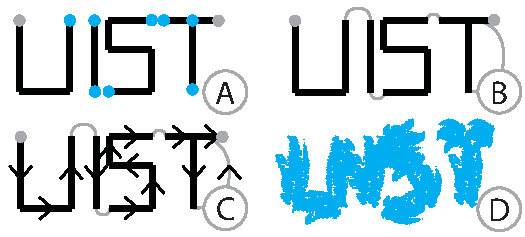
\includegraphics[width=3.4in]{figures/interior.pdf}
\caption{An input vector graphics file with the points which cannot be tubed as drawn highlighted in {\color{blue}blue} and the start and end points highlighted in {\color{gray}gray} (a).  The connected graph created by our software (b) and the resulting Euler circuit (c) permit creation of a novel neon sign (d).}
\label{fig:tool-process-interior}
\end{figure}

\begin{figure}[h!]
\centering
    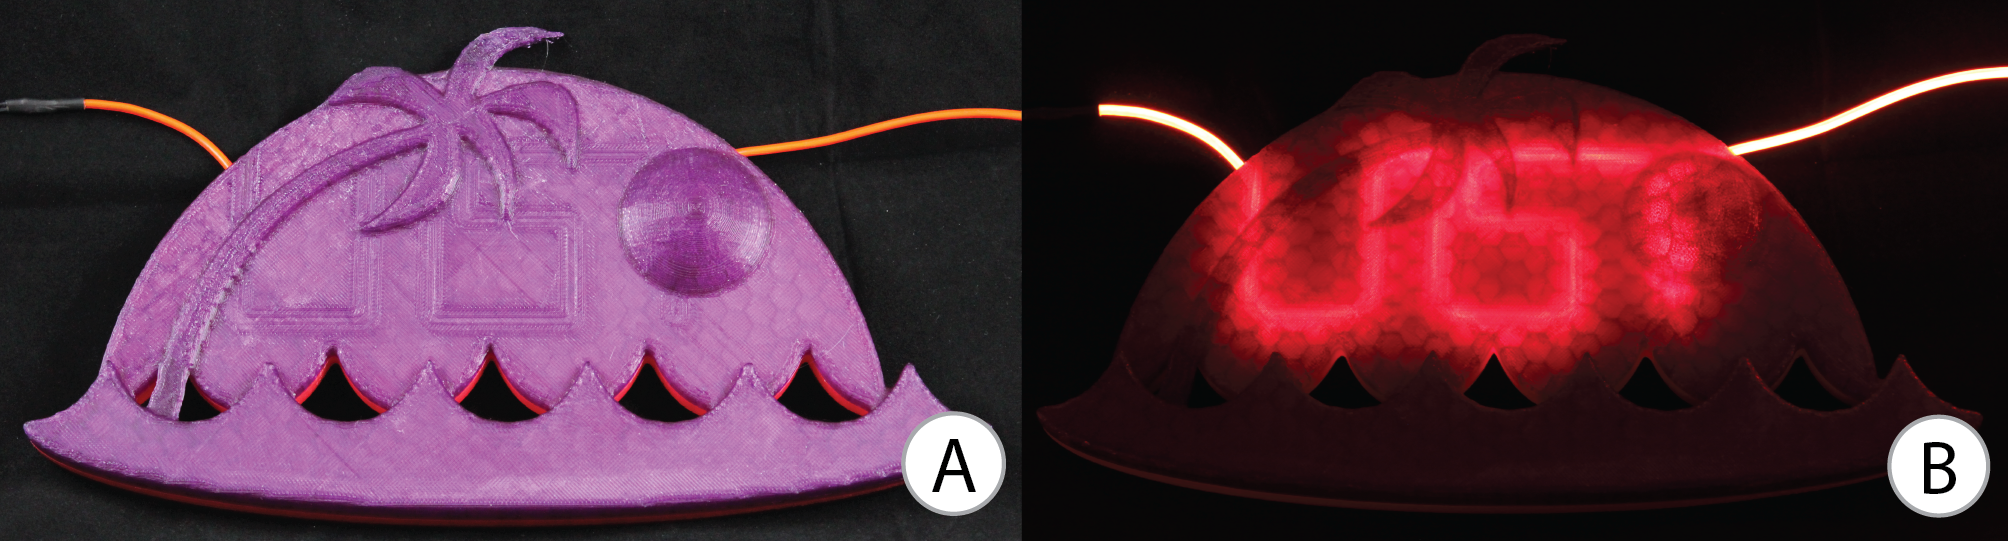
\includegraphics[width=3.4in]{figures/uistphotos.png}
\caption{Our neon sign built using the process above.  (a) shows the unlit sign, and (b) shows it lit.}
\label{fig:UIST}
\end{figure}

\subsubsection{Routing} \george{condense or just point to appendix}
To allow for a single path through a pipe for post-print media insertion, we need to find a semi-Eulerian graph of which a user's input graphics are a subset, and subsequently find an Euler tour on that graph.

The interior path routing problem is a version of the Chinese Postman Problem\footnote{The CPP is also known as the route inspection problem: \url{http://en.wikipedia.org/wiki/Route_inspection_problem}}, in which we wish to traverse all edges of the graph described in the user's input, much as a postman needs to walk along every road at least once to deliver mail.  In our relaxation, we allow creation of new edges (i.e., the postman may traverse buildings in addition to roads).  If path components are disconnected, we create edges that connect them; additionally we can create edges connecting odd-degree vertices rather than simply retracing existing edges.  In the final artifact, all created edges will be blocked out by dark material so the inserted medium is not visible (see Figure \ref{fig:tool-process-interior}).  We offer a short algorithm here, with a more mathematically precise definition and associated proof in the appendix.

In order to create a semi-Eulerian graph, we first add a temporary edge to the start and end points.  This is removed after the graph is made fully Eulerian.

To connect disconnected subgraphs in the input, each disconnected subgraph's vertices and edges are contracted to a single vertex.  Each subgraph-vertex has no outgoing edges, as the expanded subgraphs are disconnected.  We then add one edge from each subgraph-vertex to each other subgraph-vertex, whose weight is the minimum Euclidean distance between any two vertices in the expanded subgraphs.  We greedily select the smallest weight edges until all subgraphs are joined into a single graph.  We re-expand the subgraphs.

In order to make our graph Eulerian, we consider all odd degree vertices in the connected graph and make a clique of potential edges based on distance.  We greedily add edges between the odd nodes until no odd nodes remain.  Finally, we remove our temporary edge, which changes the graph from Eulerian to semi-Eulerian.  This is a connected, semi-Eulerian graph which contains all edges in the input (see Appendix).

We believe that a lower total weight matching is possible by connecting components and ensuring node evenness together in a global process, as well as by using minimum-weight matching rather than greedy selection, however this optimization is not crucial for our purposes.

/george{too complicated}
Once we have a semi-Eulerian graph, we need to create an Euler tour.  We use a weighted modification of Fleury's algorithm for finding Euler tours\footnote{\url{http://en.wikipedia.org/wiki/Eulerian_path\#Fleury.27s_algorithm}} for this.  In the classic algorithm, each selected edge is removed to create a reduced graph.  To select the next edge while at a node, the algorithm randomly chooses from all incident non-bridge edges (where a bridge edge would create disconnected non-trivial subgraphs if it were removed).  This ensures that every edge is both reachable and traversed.  In our modification, instead of randomly selecting from non-bridge paths at each node, we select the non-bridge edge which turns the least from the most recent path (i.e., we prefer to pass straight through a node, if possible).  This minimizes turns in the final artifact, which eases support material removal and assembly.  Our EL wire in Figure \ref{fig:UIST} follows an Euler tour through the input nodes.

\subsubsection{Edges that Intersect in the Plane}
We do not currently redirect edges that intersect in the plane.  Because we have a 3-dimensional canvas in which to work, it would be possible to push overlapping paths into the third dimension.  However, we leave this to future work: for our specific applications so far, it has been unnecessary.

\subsection{Mesh Modification}
Once we have a set of authored paths, we must cut tubes out of the input mesh.
Our basic strategy is to create a polygonal tube by sweeping a profile polyline
along the path, and subtract the tube from the mesh. We only use circular profiles
in our examples, but clearly any other profile could be used. Similarly our interface
allows different start and end radii, which are linearly interpolated along the path.

To avoid the complexities of direct mesh booleans, we construct a discretized volumetric
(i.e., voxel-based) representation of the original mesh and the tube mesh. Boolean
subtraction is trivial in such representations. We specifically use narrow-band
level sets~\cite{Museth04}, which represent the surface as the zero iso-contour of an
approximate distance field.
We then use marching cubes~\cite{Lorensen87} to produce the final mesh for printing.
This strategy does incur some resampling artifacts, however so does the 3D printing, and compared to the print process, the time required to voxelize at high resolution is inconsequential.
Since we have a distance field, we can easily introduce useful effects, such as the
ability to add a thin membrane ``cap'' over the end of a tube. 
This is accomplished by applying a standard ``thicken'' operation to the level set version
of the initial mesh, intersecting with a sphere placed at the tube endpoint, and then performing
a boolean union with the initial shape-minus-tube result (see Figure \ref{fig:cap}).
A straightforward extension would be to add or subtract additional elements at
the tube endpoints.

\begin{figure}[h!]
\centering
    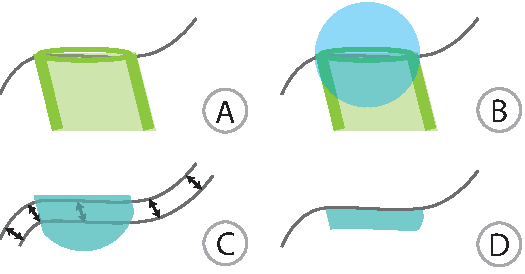
\includegraphics[width=3.4in]{figures/cap.pdf}
\caption{The process to ``cap'' the end of a pipe.  In (a), a pipe end is placed on the surface of the mesh.  In (b), we create a sphere whose radius is slightly larger than the radius of the pipe, centred at the tube's endpoint.  In (c), we consider the intersection of the sphere and the pipe, and create an offset surface of the mesh.  Finally, in (d) we intersect with the offset surface.  This is kept as a cap for the pipe in mesh subtraction.}
\label{fig:cap}
\end{figure}

\subsection{Fabrication Techniques}

Beyond design, the tubes must actually be printable to be useful.  When geometries contain overhangs, as there may be in designed pipes and cavities, 3D printers lay down support material that can be later removed from the model.  This removal process can be time-intensive and challenging.  The physical fabrication process used by different machines gives rise to differing strategies for avoiding support material or easing its removal.  We will discuss techniques for fused deposition modeling (FDM) machines like the Makerbot and multi-jetting machines like the Objet.

FDM machines lay down lines of plastic on top of each other: this allows ``stepover'', when a layer of plastic is laid slightly offset from the layer below it, and ``bridging'', when plastic is laid across a gap between two surfaces.  For a layer to fix correctly to its supporting layer, roughly half of the filament needs to overlap.  This means that overhangs without added support material can be approximately $45^{\circ}$, and although cylinders (e.g., pipes) and spheres violate this in some places they are printable support-free.  Support is made from the same material as the model, laid in a heatsink-like wave pattern.  It is straightforward to remove from exterior surfaces with fingers or pliers, but nearly impossible to remove from internal cavities.  Meshmixer has a built-in tool for minimizing support for FDM prints; it re-orients the part to keep as much surface area as possible within the 45 degree constraint.  In future work we would like to explore a tool in which a user can select surfaces to prioritize support avoidance for.  

On multi-jetting machines, bridging is not possible and stepover potential is much less, because the machine is laying down droplets of liquid rather than more structural plastic.  Unsupported overhangs can be approximately $14^{\circ}$.  The support structure used by this machine is a loose matrix of material that can be removed by hand from the surface, blasted out with a water jet from cavities, or dissolved in lye (the enclosing model material does not dissolve).  Thus, any cavity to which there is some access can be cleared of support.

For especially complex geometries, models can be ``cut up'' into assembleable pieces that evade support requirements or ease material removal.  This is undesirable as it means more time spent in assembly post-print, and additionally a cut pipe may not be fluid-tight any longer.  An automatic tool for this task might be beneficial, however it is outside the scope of this work.
